\documentclass{article}
\usepackage{tikz}
\usetikzlibrary{arrows.meta, positioning}

\begin{document}

\begin{figure}[h]
    \centering
    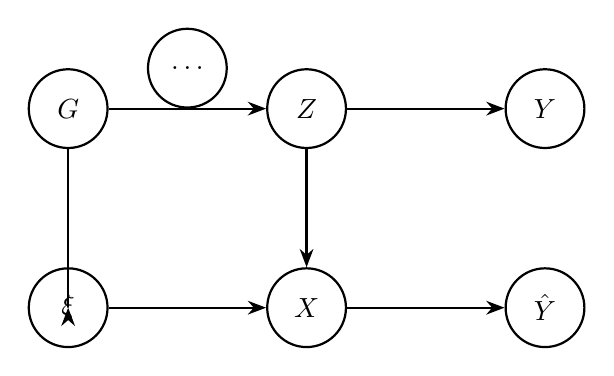
\begin{tikzpicture}[
        node distance = 15mm and 20mm,
        every node/.style = {circle, draw, minimum size=1cm},
        >=Stealth,
        thick,
        every label/.append style = {font=\small},
        ]
        % Nodes
        \node (G) {$G$};
        \node[below=of G] (xi) {$\xi$};
        \node[right=of G] (Z) {$Z$};
        \node[right=of Z] (Y) {$Y$};
        \node[below=of Z] (X) {$X$};
        \node[right=of X] (Yhat) {$\hat{Y}$};

        % Edges
        \draw[->] (G) -- node[above] {$\dots$} (Z);
        \draw[->] (G) |- (xi);
        \draw[->] (Z) -- (Y);
        \draw[->] (Z) -- (X);
        \draw[->] (xi) -- (X);
        \draw[->] (X) -- (Yhat);
    \end{tikzpicture}
    \caption{
        We study a prediction model on feature vectors with differential under-reporting $X$ where true outcomes $Y$ are a function of the latent `true' features $Z$. Missingness $\xi$ is influenced by group membership $G$. We consider both cases in which feature distributions vary by group membership and cases with $G \perp Z$. In our setting, missingness indicators $\xi$ are unobserved and group membership $G$ is only used for model evaluation and not as a feature. The graph reflects the dependencies at prediction time.
    }
    \label{fig:prediction_model}
\end{figure}

\end{document}